\documentclass{main.tex}[subfiles]
\begin{document}
\section{Вычислительные эксперименты}
\subsection{Предобработка данных и выравнивание}
% TODO images

\begin{figure}[H]
    \centering
    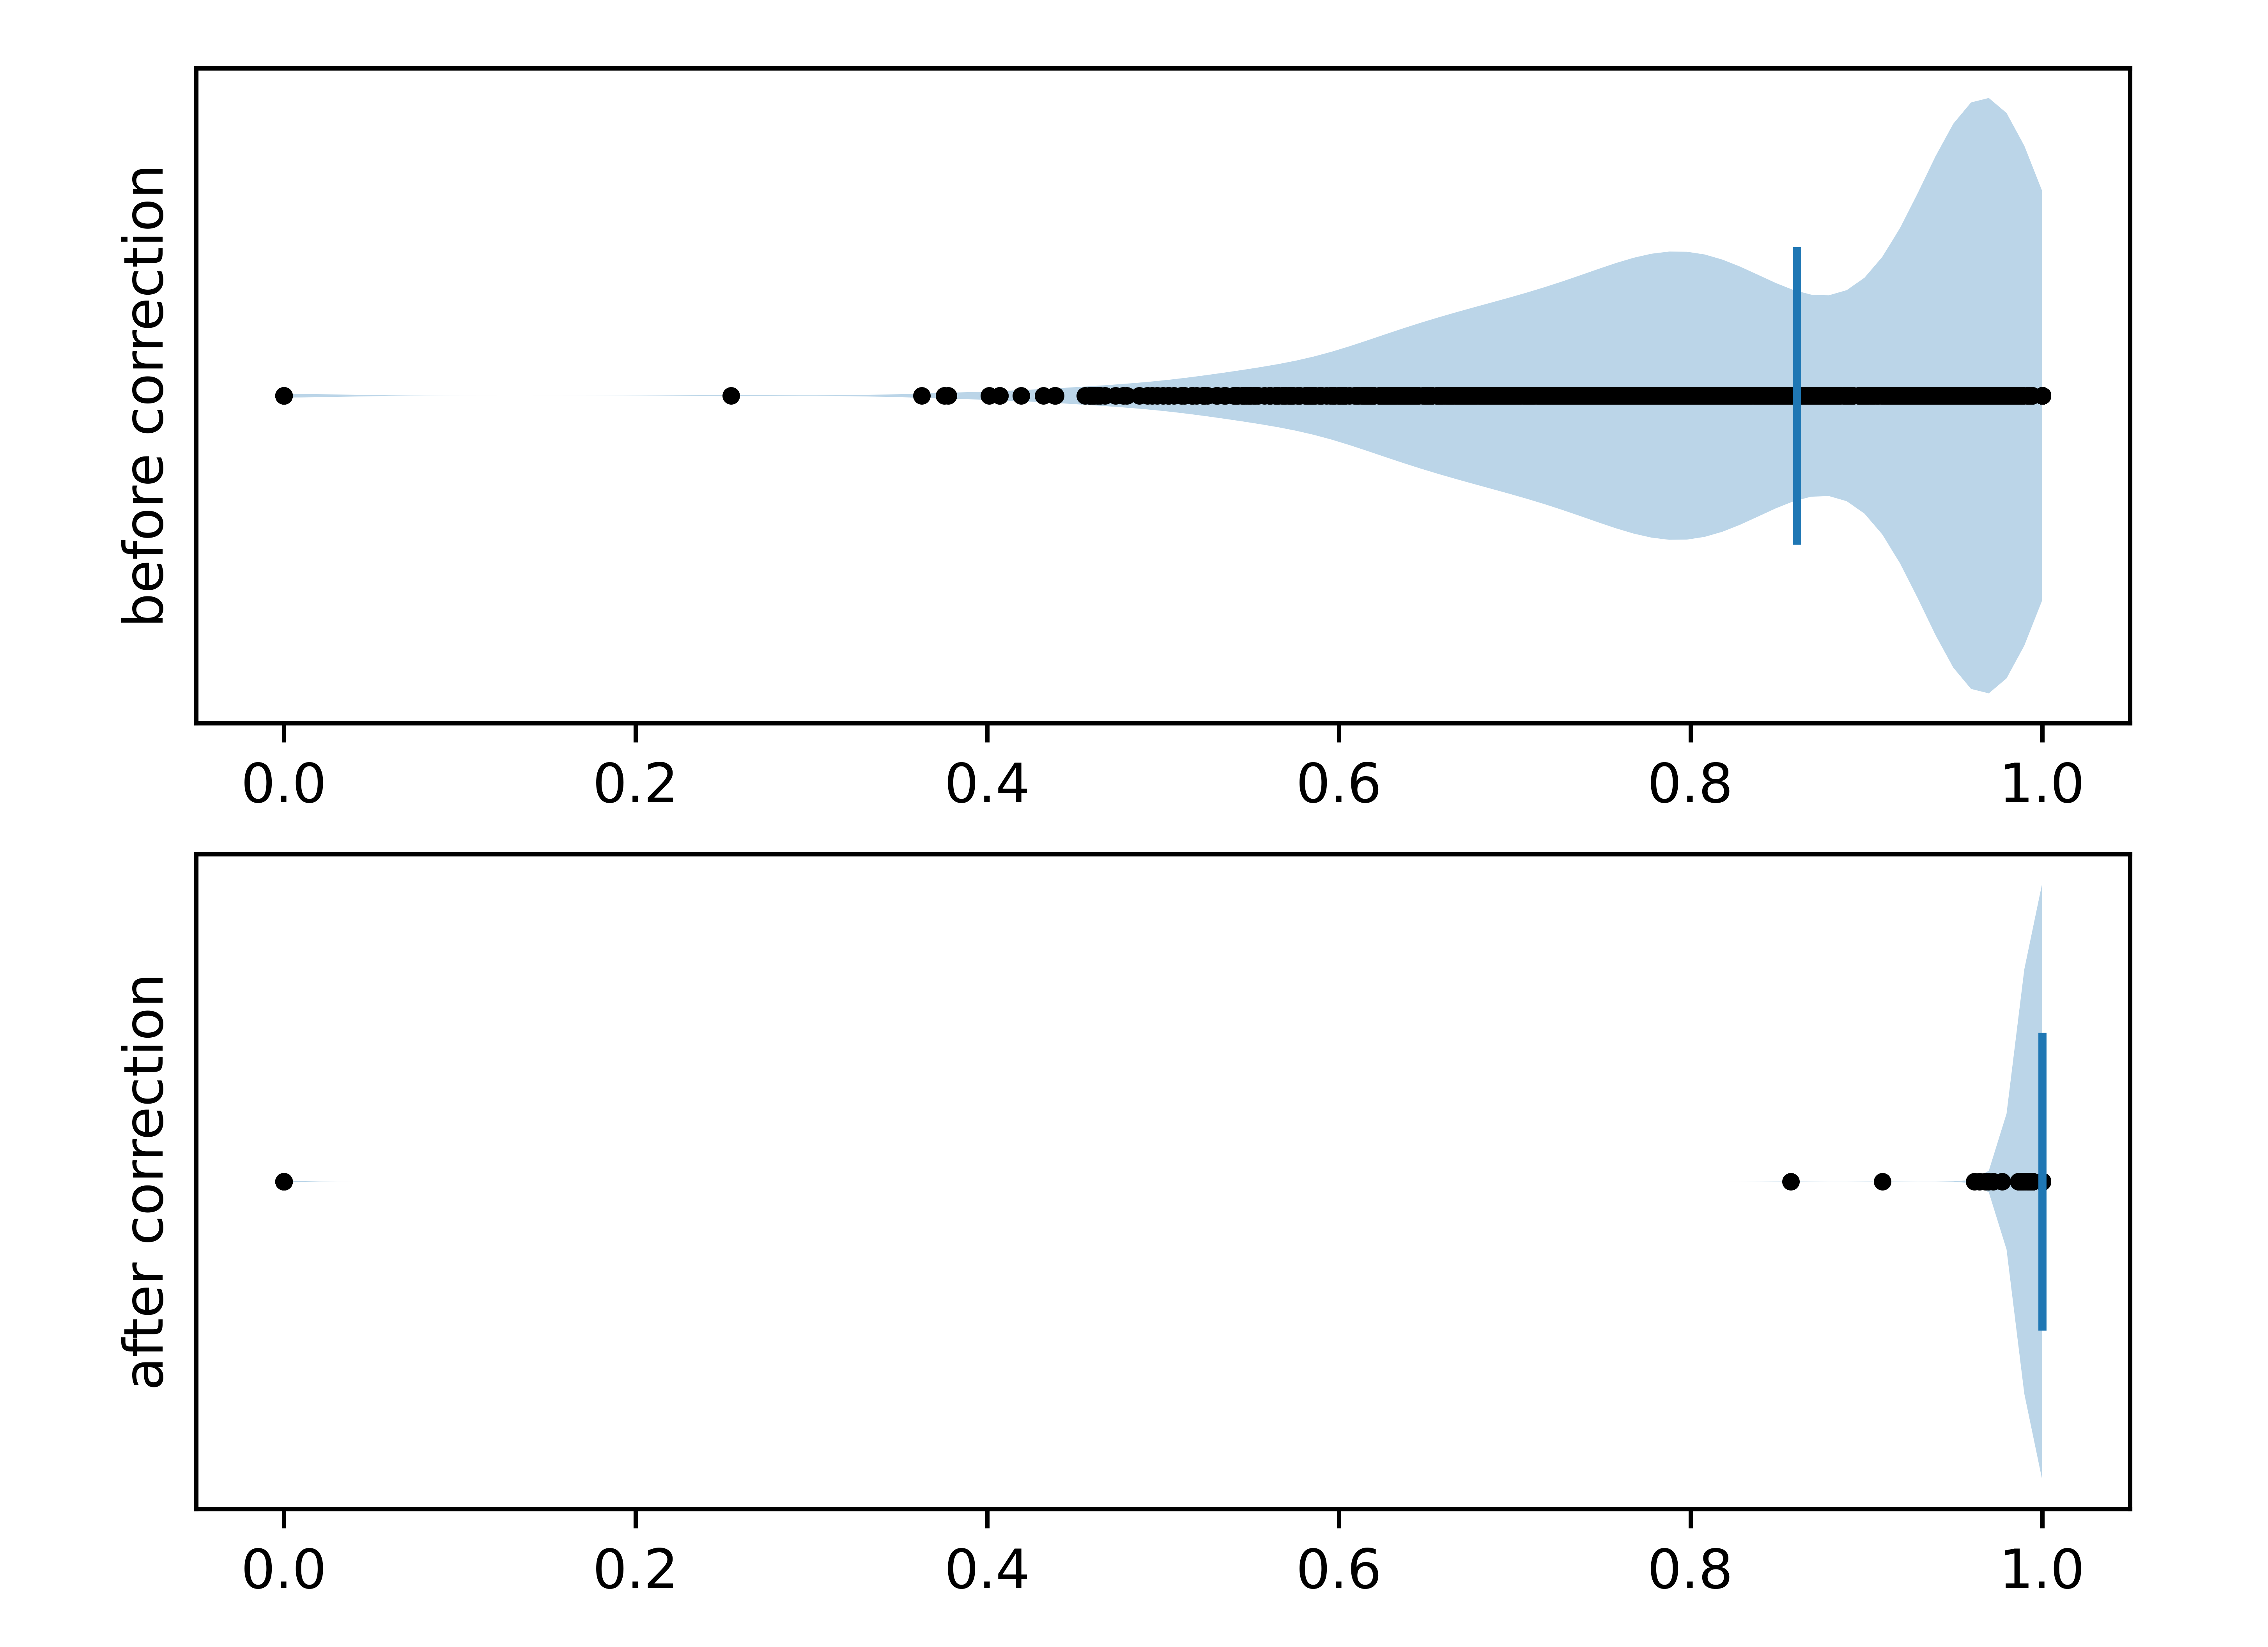
\includegraphics[width=\myPictWidth]{frequencies}
    \caption{Доля слов в распознанном тексте, встречающихся в исходном: до выравнивания (вверху) и после (внизу). Чёрные точки -- элементы выборки, голубая область -- ядерная оценка плотности распределения с ядром Гаусса (т. н. violinplot), синяя вертикальная черта -- медиана выборки}
    \label{fig:frequencies} % TODO ref in the text
\end{figure}

\subsection{Обучение нейронной сети}
\end{document}